\documentclass[11pt,aspectratio=1610]{beamer}

\usetheme[
    background=light,
    numbering=fraction,
    block=fill,
    progressbar=frametitle
]{metropolis}
\usepackage{appendixnumberbeamer}

\usepackage{wasysym}
\usepackage{booktabs}
\usepackage{physics}
\usepackage{amsmath}
\usepackage{mathtools}
\usepackage{bm}
\usepackage{tcolorbox}
\newtcolorbox{idea}{colback=green!5!white,colframe=green!75!black}
\newtcolorbox{warning}{colback=red!5!white,colframe=red!75!black}

\usepackage{tikz}
\usetikzlibrary{quantikz}

\usefonttheme[onlymath]{serif}
\usefonttheme{professionalfonts}
\usepackage{unicode-math}

\defaultfontfeatures{ Scale=MatchLowercase }
% \setmainfont{TeX Gyre Pagella}[Scale = 1.0]
\setmathfont{Asana Math}
% \setmathfont{Neo Euler}[
%   range={up/{Latin, latin, Greek, greek},
%          bfup/{Latin, latin, Greek, greek},
%          cal, bfcal,
%          frak, bffrak
%         },
%   script-features={},
%   sscript-features={} ]


\newcommand{\iu}{\mathrm{i}\mkern1mu}
\newcommand{\unitary}[1]{\raisebox{-1pt}{\scalebox{1.2}{$\bm{\mathsf{U}}$}}\qty(#1)}


\title{The Gottesman-Knill Theorem}
\subtitle{What is it and what does it mean?}
\date{10/12/2020}
\author{Nate Stemen (he/they)}
\institute{QIC 710 Final Project}
\titlegraphic{\hfill
\includegraphics[height=2cm]{uw-logo-blue.png}}


\begin{document}

\maketitle

\begin{frame}{The Gottesman-Knill Theorem}
	\begin{theorem}[\cite{gottesman-knill}]
		A quantum circuit using only the following elements can be efficiently \textbf{simulated} on a classical computer:
		\begin{enumerate}
			\item Qubits prepared in computational basis states
			\item Quantum gates from the \textbf{Clifford group}
			\item Measurements in the computational basis
		\end{enumerate}
	\end{theorem}
\end{frame}

\begin{frame}{What does a classical simulation of a quantum computer mean?}
	Two different main kinds of simulation possible:\pause
	\begin{exampleblock}{Strong Simulation}
		Given an input $x$ to our quantum computer, compute $p(x)$.
	\end{exampleblock}\pause
	\begin{exampleblock}{Weak Simulation}
		Given an input $x$, compute a sample from $p(x)$.
	\end{exampleblock}\pause
	Gottesman-Knill theorem deals with weak simulation.

	Strong simulation of quantum computers shown to be $\#\bm{\mathsf{P}}$-hard \cite{nest}.
\end{frame}

\begin{frame}[t]{How can we (na\"ively) simulate a quantum computer?}
	Suppose we have $n$ qubits and we want to run them through $D$ gates.
	\begin{center}
		\begin{quantikz}
			\lstick[wires=3]{$\mathbb{C}^{2^n}\ni \ket{\psi}$} & \gate[wires=3]{A_1} & \gate[wires=3]{A_2} & \ \ldots\ \qw &  \gate[wires=3]{A_D} & \qw \rstick[wires=3]{$A_D\cdots A_2A_1\ket{\psi}$} \\
			& \qwbundle[alternate]{}  &  \qwbundle[alternate]{}     & \ \ldots\ \qwbundle[alternate]{} & \qwbundle[alternate]{} & \qwbundle[alternate]{} \\
			&                     &                          & \ \ldots\ \qw & & \qw
		\end{quantikz}
	\end{center}

	\begin{onlyenv}<1>
		Final state contains $D-1$ matrix multiplications, each costing $O\qty(2^{3n})$\footnote{Theoretically possible to get $O\qty(2^{2.373 n})$.}, so total cost is $O\qty(D2^{3n})$.

		Simulating Grover's algorithm on 40 qubits took nearly a full day! \cite{slowsim}
	\end{onlyenv}
	\begin{onlyenv}<2>
		\begin{idea}
			\begin{center}
				What if we restrict the gates $A_i$?
			\end{center}
		\end{idea}
	\end{onlyenv}

\end{frame}

\section{Stabilizer Formalism}

\begin{frame}{Stabilizer Formalism}
	\begin{itemize}[<+->]
		\item Let $\ket{\psi} = \frac{1}{\sqrt{2}}\qty(\ket{00} + \ket{11})$
		\item $X_1X_2\ket{\psi} = \ket{\psi}$ and $Z_1Z_2\ket{\psi} = \ket{\psi}$
		\item $\ket{\psi}$ is the \emph{unique} state stabilized by both of these operators.
		\item This hints at the possibility of describing some states not as vectors in $\mathbb{C}^{2^N}$, but of operators.
	\end{itemize}
\end{frame}

\begin{frame}[t]{Pauli Group}
	Let $X, Y, Z$ denote the standard single-qubit Pauli operators:
	\begin{align*}
		X & = \mqty(0 & \phantom{+}1 \\ 1 & \phantom{+}0) & Y & = \mqty(0 & -\iu \\ \iu & \phantom{-}0) & Z & = \mqty(1 & \phantom{-}0 \\ 0 & -1)
	\end{align*}
	\begin{onlyenv}<2->
		Take $X_i, Y_i, Z_i$ to denote $X, Y$ and $Z$ acting on the $i$-th qubit, and with the identity everywhere else.
	\end{onlyenv}
	\begin{onlyenv}<2>
		\begin{columns}
			\begin{column}{0.7\textwidth}
				\begin{equation*}
					X_i\coloneqq \mathbb{1}\otimes\cdots\otimes\overbrace{X}^{i\text{th operator}}\otimes \cdots \otimes \mathbb{1}
				\end{equation*}
			\end{column}
			\begin{column}{0.3\textwidth}
				\vspace{-0.8cm}
				\begin{quantikz}
					\lstick{$1$} & \qw & \qw \\
					\lstick{$\vdots$} & \qwbundle[alternate]{} & \qwbundle[alternate]{} \\
					\lstick{$i$} & \gate{X} & \qw \\
					\lstick{$\vdots$} & \qwbundle[alternate]{} & \qwbundle[alternate]{} \\
					\lstick{$n$} & \qw & \qw \\
				\end{quantikz}
			\end{column}
		\end{columns}
	\end{onlyenv}

	\begin{onlyenv}<3>
		\begin{equation*}
			P_n\coloneqq\qty{\pm\mathbb{1}, \pm\iu\mathbb{1}, \pm A_i, \pm\iu A_i: A_i\in\{\mathbf{1}, X_i, Y_i, Z_i\}}\equiv \langle X_i, Z_i\rangle
		\end{equation*}
		\begin{itemize}
			\item $P_n$ forms a group under matrix multiplication.
			\item Every pair of elements either commute or anti-commute.
			\item $\abs{P_n} = 4\cdot 4^n$
		\end{itemize}
	\end{onlyenv}
\end{frame}

\begin{frame}{Stabilizer States}
	Let $S$ be a subgroup of $P_n$. Define the \emph{vector space} $V_S$ as the states stabilized by everything in $S$.
	\begin{equation*}
		V_S\coloneqq \qty{\ket{\psi}\in\mathbb{C}^{2^n}: g\ket{\psi} = \ket{\psi}, \forall g\in S}
	\end{equation*}
	\begin{exampleblock}{Example}
		Take $P_3$ and subgroup $S = \qty{\mathbb{1}, Z_1Z_2, Z_2Z_3, Z_1Z_3}$. Note that $\ket{000}, \ket{001}, \ket{110}, \ket{111}$ are stabilized by $Z_1Z_2$, and $\ket{000}, \ket{100}, \ket{011}, \ket{111}$ are stabilized by $Z_2Z_3$. These, together with the fact that $Z_1Z_3 = (Z_1Z_2)(Z_2Z_3)$ tell us that $V_S = \qty{\ket{000}, \ket{111}}$. In this case we can write $S = \langle Z_1Z_2, Z_2Z_3\rangle$.
	\end{exampleblock}
	\onslide<2->{\begin{idea}\begin{center}$S$ and $V_S$ uniquely determine each other!\end{center}\end{idea}}
\end{frame}

\begin{frame}[t]{What about other gates?}
	Let $U$ by an arbitary unitary gate from $\unitary{2^n}$, $\ket{\psi}\in V_S$ and $g\in S$.\pause
	\begin{equation*}
		U\ket{\psi} = Ug\ket{\psi} = UgU^\dagger U\ket{\psi} = g'U\ket{\psi}
	\end{equation*}\pause
	So $U\ket{\psi}$ is stabilized by $UgU^\dagger$, and in general $UV_S$ is stabilized by $USU^\dagger = \qty{UgU^\dagger : g\in S}$.

	\begin{corollary}
		If $S$ is generated by $g_1,\ldots, g_n$, then $USU^\dagger$ is generated by $Ug_1U^\dagger,\ldots, Ug_nU^\dagger$.
	\end{corollary}\pause

	If $G$ is an Abelian group with $\abs{G}$ the number of elements in $G$, then the number of generators of $G$ is bounded by $\log\abs{G}$.\pause

	\begin{warning}
		\begin{center}
			What if $UgU^\dagger$ doesn't land back in $P_n$?
		\end{center}
	\end{warning}
\end{frame}

\begin{frame}[t]{Clifford Group}
	\only<1-2>{
		\begin{warning}
			\begin{center}
				What if $UgU^\dagger$ doesn't land back in $P_n$?
			\end{center}
		\end{warning}}

	\begin{theorem}
		Suppose $U$ in any unitary on $n$ qubits with the property that for $g\in P_n$ we have $UgU^\dagger\in P_n$. Then $U$ can be composed from $O(n^2)$ Hadamard, CNOT, and phase gates.
	\end{theorem}\pause

	\begin{block}{Definition}
		The \emph{Clifford Group} is defined to be the set of operators that leave Pauli operators invariant under conjugation.
		\begin{equation*}
			C_n \coloneqq \qty{V\in \unitary{2^n} : VP_nV^\dagger = P_n}
		\end{equation*}
	\end{block}
	\onslide<3>{\begin{align*}
			H & = \frac{1}{\sqrt{2}}\mqty(1 & \phantom{-}1 \\ 1 & -1) & P & = \mqty(1 & \phantom{+}0 \\ 0 & \phantom{+}\iu) & \textbf{CNOT}
		\end{align*}}
\end{frame}

\begin{frame}{Recap}
	\begin{enumerate}[<+->]
		\item Simulating a quantum computer in general is \emph{really} hard!
		\item What can we simulate more easily?
		\item Stabilizer formalism gave us a way to track operators instead of state vectors (duality between subgroup $S$ of Paulis and vector space of stabilised states $V_S$)
		\item Keeping track of the generators of a stabilizer $S$ provide a succinct way to understand how $S$ is changing ($\log\abs{S}$ generators)
		\item Found that elements of the Clifford group can efficiently build elements that conjugate the Pauli group back to the Pauli group
	\end{enumerate}
\end{frame}

\begin{frame}[t]{Example}
	\begin{columns}[T,onlytextwidth]
		\column{0.8\textwidth}
		\begin{exampleblock}{Alice's Broken Quantum Computer \frownie}
			Alice's quantum computer is working too well. Instead of performing single controlled-NOT gates, it does three at a time. What is it actually doing?
		\end{exampleblock}

		\column{0.2\textwidth}
		\begin{center}
			\begin{quantikz}
				& \ctrl{1}  & \targ{}   & \ctrl{1} & \qw \\
				& \targ{}   & \ctrl{-1} & \targ{}  & \qw
			\end{quantikz}
		\end{center}
	\end{columns}

	\onslide<2->{Because $X_1, X_2, Z_1, Z_2$ generate the Pauli group we can follow what happens to them under the evolution of this circuit.}
	\begin{align*}
		\only<2>{X_1     & = X\otimes\mathbb{1} \xrightarrow{\text{CNOT 1}} \text{CNOT}\cdot \qty(X\otimes\mathbb{1}) \cdot\text{CNOT}^\dagger = X\otimes X\\}
		\onslide<3->{X_1 & = X\otimes\mathbb{1}\xrightarrow{\text{CNOT 1}}X\otimes X\xrightarrow{\text{CNOT 2}}\mathbb{1}\otimes X\xrightarrow{\text{CNOT 3}}\mathbb{1}\otimes X = X_2 \\}
		\onslide<3->{Z_1 & = Z\otimes\mathbb{1}\xrightarrow{\text{CNOT 1}}Z\otimes \mathbb{1}\xrightarrow{\text{CNOT 2}}Z\otimes Z\xrightarrow{\text{CNOT 3}}\mathbb{1}\otimes Z = Z_2}
	\end{align*}
	\onslide<3->{Further, we can show $X_1\longleftrightarrow X_2$ and $Z_1\longleftrightarrow Z_2$. This is exactly a swap operation!}
\end{frame}

\begin{frame}[t]{Example, continued}
	\begin{columns}[T,onlytextwidth]
		\column{0.8\textwidth}
		\begin{exampleblock}{Alice's less Broken Quantum Computer \smiley}
			By dint of no little hard work, Alice has partially fixed her quantum computer. Now it only does 2 CNOTs at a time. Unfortunately, she can only get this improvement if she puts a $\ket{0}$ as the second input qubit. What does it do now?
		\end{exampleblock}

		\column{0.2\textwidth}
		\vspace{.5cm}
		\begin{center}
			\begin{quantikz}
				\lstick{$\ket{\alpha}$} & \ctrl{1} & \targ{} & \qw \\
				\lstick{$\ket{0}$}      & \targ{}  & \ctrl{-1}  & \qw
			\end{quantikz}
		\end{center}
	\end{columns}
	In this case we see the initial state $\ket{\psi_0} = \ket{\alpha}\otimes\ket{0}$ is stabilized by $Z_2$.
	\only<2>{\begin{align*}
			X_1 & = X\otimes\mathbb{1}\xrightarrow{\text{CNOT 1}}X\otimes X\xrightarrow{\text{CNOT 2}}\mathbb{1}\otimes X \\
			Z_1 & = Z\otimes\mathbb{1}\xrightarrow{\text{CNOT 1}}Z\otimes \mathbb{1}\xrightarrow{\text{CNOT 2}}Z\otimes Z \\
			Z_2 & = \mathbb{1}\otimes Z\xrightarrow{\text{CNOT 1}}Z\otimes Z\xrightarrow{\text{CNOT 2}}Z\otimes\mathbb{1}
		\end{align*}}
	\onslide<3->{\begin{align*}
			X_1 & \longrightarrow \mathbb{1}\otimes X & Z_1 & \longrightarrow Z\otimes Z & Z_2 & \longrightarrow Z\otimes\mathbb{1}
		\end{align*}}
	State will always be a $+1$ eigenvector of $Z_2$, so it follows that $(Z\otimes\mathbb{1})(Z\otimes Z) = \mathbb{1}\otimes Z$.
	\onslide<4->{\begin{align*}
			X_1 & \longrightarrow \mathbb{1}\otimes X & Z_1 & \longrightarrow \mathbb{1}\otimes Z
		\end{align*}}
	Circuit still performs a swap!
\end{frame}

\begin{frame}{Back to the Theorem}
	\begin{theorem}[\cite{gottesman-knill}]
		A quantum circuit using only the following elements can be efficiently simulated on a classical computer:
		\begin{enumerate}
			\item Qubits prepared in computational basis states
			\item Quantum gates from the Clifford group
			\item Measurements in the computational basis
		\end{enumerate}
	\end{theorem}
	\begin{itemize}
		\item Take $\ket{\psi} = \ket{0}^{\otimes n}$. Now we can say $S = \langle Z_1, \ldots, Z_n\rangle$.
		\item Under some action $U\in C_n$ state will evolve to $U\ket{\psi} = UgU^\dagger U\ket{\psi}$ for $g\in S$
		\item Switch over to describing the change in generators of $S$
		\item Need to compute $UZ_1U^\dagger,\ldots, UZ_nU^\dagger$
	\end{itemize}

\end{frame}

\begin{frame}{Back to the Theorem}
	\begin{itemize}
		\item Take $\ket{\psi} = \ket{0}^{\otimes n}$. Now we can say $S = \langle Z_1, \ldots, Z_n\rangle$.
		\item Under some action $U\in C_n$ state will evolve to $U\ket{\psi} = UgU^\dagger U\ket{\psi}$ for $g\in S$
		\item Switch over to describing the change in generators of $S$
		\item Need to compute $UZ_1U^\dagger,\ldots, UZ_nU^\dagger$
		\item Only takes $2n+1$ bits to keep track of the generators: 2 for the $n$ Pauli generators, and 1 for the phase of $\pm 1$
		\item Thus to specify $\ket{\psi}$ it takes $n(2n+1)$ bits, and updating the generators only takes $O(n)$
	\end{itemize}
\end{frame}

\begin{frame}[t]{What does this mean?}
	What makes quantum computers powerful?\pause
	\begin{warning}
		\begin{center}
			Not entanglement!
		\end{center}
	\end{warning}\pause
	\only<3>{Circuits built with the Clifford group don't actually provide us with any more power than a classical computer, despite CNOTs, Hadamards, and phase gates being used to construct purely quantum phenomenon.}
	\onslide<4->{\begin{columns}
			\begin{column}{0.2\textwidth}
				\only<4>{Quantum teleportation}
				\only<5>{Superdense coding}
			\end{column}
			\begin{column}{0.8\textwidth}
				\begin{center}
					\only<4>{\begin{quantikz}[row sep=0.8cm]
							\lstick{$\ket{\psi}$} & \qw & \qw & \ctrl{1}\gategroup[2,steps=5,style={dashed,rounded corners,fill=blue!20, inner xsep=2pt},background, label style={label position=above,yshift=-1.7cm, xshift=0.4cm}]{Alice}   & \gate{H} & \meter{$M_1$}  & \cw & \cwbend{2}    \\
							\lstick{$\ket{0}$} & \gate{H} & \ctrl{1} & \targ{}  & \qw & \meter{$M_2$} & \cwbend{1}           \\
							\lstick{$\ket{0}$} & \qw      & \targ{} & \qw \gategroup[1,steps=5,style={dashed,rounded corners,fill=green!20, inner xsep=2pt},background, label style={label position=below,xshift=-0.3cm}]{Bob}     & \qw & \qw & \gate{X^{M_2}} & \gate{Z^{M_1}} & \qw \rstick{$\ket{\psi}$}
						\end{quantikz}}
					\only<5>{\begin{quantikz}[row sep=0.8cm]
							\lstick{$\ket{0}$} & \gate{H} & \ctrl{1} & \gate{X^a} & \gate{Z^b} & \ctrl{1} & \gate{H} & \meter{} & \cw\rstick{$a$} \\
							\lstick{$\ket{0}$} & \qw      & \targ{}  & \qw      & \qw      & \targ{}  & \qw      & \meter{} & \cw\rstick{$b$}
						\end{quantikz}}
				\end{center}
			\end{column}
		\end{columns}}
\end{frame}

\begin{frame}{Where do we go from here?}
	\begin{itemize}[<+->]
		\item Clifford gates aren't enough for universal quantum computation
		\item Clifford group shown to be $\oplus\bm{\mathsf{L}}$-complete \cite{aaronson}
		\item Adding \emph{any} 1 or 2-qubit gate\footnote<3->{That doesn't map computational basis states to computational basis states} will turn the Cliffords into a universal set \cite{shi}
	\end{itemize}
	\onslide<2->{\begin{center}
			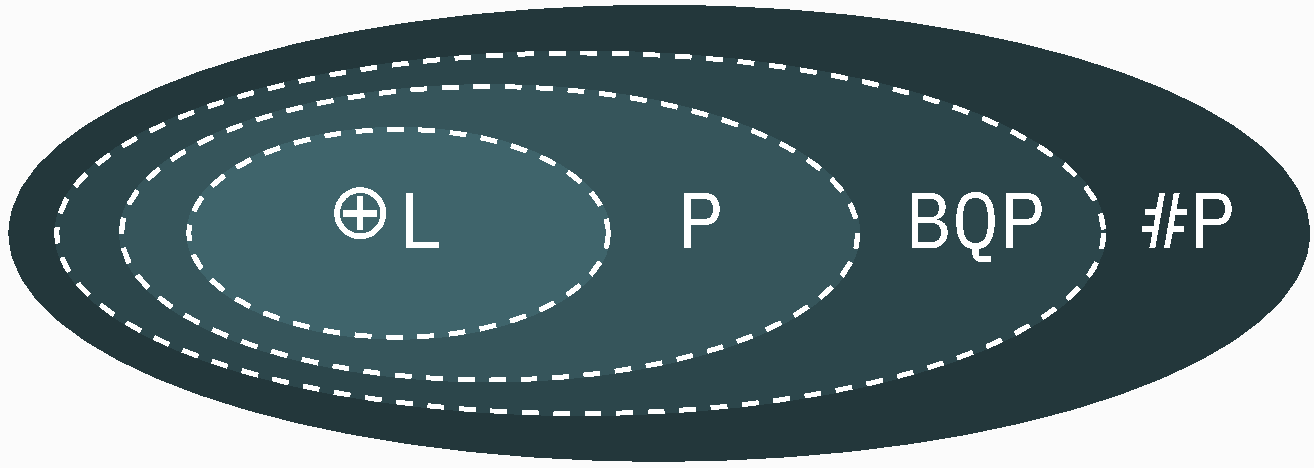
\includegraphics[width=0.65\textwidth]{complexity.pdf}
		\end{center}}
\end{frame}

\begin{frame}[allowframebreaks]{References}
	\nocite{*}
	\bibliographystyle{apalike}
	\bibliography{refs}
\end{frame}

\begin{frame}[standout]
	\smiley Thank you!\smiley

	Questions?
\end{frame}

\end{document}
